%%%%%%%%%%%%%%%%%%%%%%%%%%%%%%%%%%%%%%%%%%%%%%%%%%%%%%%%%%%%%%%%%%%%%%%%%%%%%%%%
% WeBWorK Online Homework Delivery System
% Copyright � 2000-2007 The WeBWorK Project, http://openwebwork.sf.net/
% $CVSHeader: webwork2/conf/snippets/hardcopyPreamble.tex,v 1.3 2005/09/17 20:12:01 gage Exp $
% 
% This program is free software; you can redistribute it and/or modify it under
% the terms of either: (a) the GNU General Public License as published by the
% Free Software Foundation; either version 2, or (at your option) any later
% version, or (b) the "Artistic License" which comes with this package.
% 
% This program is distributed in the hope that it will be useful, but WITHOUT
% ANY WARRANTY; without even the implied warranty of MERCHANTABILITY or FITNESS
% FOR A PARTICULAR PURPOSE.  See either the GNU General Public License or the
% Artistic License for more details.
%%%%%%%%%%%%%%%%%%%%%%%%%%%%%%%%%%%%%%%%%%%%%%%%%%%%%%%%%%%%%%%%%%%%%%%%%%%%%%%%

\batchmode
\documentclass[10pt,dvips]{amsart}
\usepackage{amsmath,amsfonts,amssymb,multicol}
\usepackage[pdftex]{graphicx}
\usepackage{epstopdf}  % allows use of eps files with pdftex
\usepackage{epsf}
\usepackage{epsfig}
\usepackage{pslatex}
\pagestyle{plain}
\textheight 9in
\oddsidemargin = -0.42in
\evensidemargin = -0.42in
\textwidth= 7.28in
\columnsep = .25in
\columnseprule = .4pt
\def\endline{\bigskip\hrule width \hsize height 0.8pt }
\newcommand{\lt}{<}
\newcommand{\gt}{>}
\newcommand{\less}{<}
\newcommand{\grt}{>}

% BEGIN capa tex macros

\newcommand{\capa}{{\sl C\kern-.10em\raise-.00ex\hbox{\rm A}\kern-.22em%
{\sl P}\kern-.14em\kern-.01em{\rm A}}}
  
\newenvironment{choicelist}
{\begin{list}{}
	{\setlength{\rightmargin}{0in}\setlength{\leftmargin}{0.13in}
	\setlength{\topsep}{0.05in}\setlength{\itemsep}{0.022in}
	\setlength{\parsep}{0in}\setlength{\belowdisplayskip}{0.04in}
	\setlength{\abovedisplayskip}{0.05in}
	\setlength{\abovedisplayshortskip}{-0.04in}
	\setlength{\belowdisplayshortskip}{0.04in}}
	}
{\end{list}}

% END capa tex macros 

\begin{document}
\voffset=-0.8in
\newpage
\setcounter{page}{1}
\begin{multicols}{2}
\columnwidth=\linewidth
%% decoded old answers, saved. (keys = 
 \end{multicols}
\noindent {\large \bf Michael Gage}
\hfill
\noindent {\large \bf MAA Minicourse New Orleans January 2001}
\par
\noindent WeBWorK assignment number MAAtutorial due 01/01/2005 at 02:00am EST;.
\hrule

\leavevmode\\\relax 
\leavevmode\\\relax 
Welcome to the MAA short course on {\bf  WeBWorK }.
\par 
Here is a synopsis of the tutorial examples presented in this set. They have been designed for learning the PG language, and are not necessarily the best questions to use for mathematics instruction.
\par 
{\bf  1. Hello world example: } Illustrates the basic structure of a PG problem.
\par 
{\bf  2. Standard example:   } This covers what you need to know to ask the majority of the questions you would want to ask in a calculus course.  Problems with text answers, numerical answers and answers involving expressions are covered.
\par 
{\bf  3. Simple multiple choice example: } Uses lists(arrays) to implement a multiple choice question.
\par 
{\bf  4. Multiple choice example: } Uses the multiple choice object to implement a multiple choice question.
\par  
{\bf  5. Matching list example: }
\par 
{\bf  6. True/false example:  }
\par 
{\bf  7. Pop-up true/false example: } Answers are chosen from a pop-up list.
\par 
{\bf  8. On-the-fly graphics example 1: } The graphs are regenerated each time you press the submit button
\par 
{\bf  9. On-the-fly-graphics example 2: } -- Adds some randomization to the first example.
\par 
{\bf  10. Static graphics example: } Presents graphs created on a separate application (e.g. Mathematica) and saved.
\par 
{\bf  11. Hermite graph example: } A particularly useful way of generating predictable graphs by specifying the value and first derivative of a function at each point.  Piecewise linear graphs are also included in this example.
\par 
{\bf  12. HTML links example: } Shows how to link other web resources to your WeBWorK problem.
\par 
{\bf  13. JavaScript example 1: } An example which takes advantage of this interactive media! This one requires students to calculate the derivative of a function from the definition.
\par 
{\bf  14. JavaScript example 2: } A variant of the previous example that generates the example function as a cubic spline so that students can't read the javaScript code to find out the answer.
\par 
{\bf  15. Vector field example } Generates vector field graphs on-the-fly.
\par 
{\bf  16. Conditional question example: } Illustrates how you can create a problem which  first asks an easy question, and once that has been answered correctly, follows up with a more involved question on the same material.
\par 
{\bf  17 Java applet example: } A preliminary example of how to include Java applets in WeBWorK problems.
\par\hrulefill\par 

The primary purpose of WeBWorK is to let you know if you are getting the right answer or to alert
you if you get the wrong answer. Usually you can attempt a problem as many times as you want before
the due date.  However, if you are having trouble figuring out your error, you should
consult the book, or ask a fellow student, one of the TA's or
your professor for help.  Don't spend a lot of time guessing -- it's not very efficient or effective.
The computer has NO CLUE about WHY your answer is wrong. Computers are good at checking,
but for help go to a human.

\par 
Give 4 or 5  significant digits for (floating point) numerical answers.
For most problems when entering numerical answers, you can if you wish
enter elementary expressions such as \(2\wedge3\) instead of 8, \(sin(3*pi/2)\)instead
of -1, \(e\wedge (ln(2))\) instead of 2,
\((2+tan(3))*(4-sin(5))\wedge6-7/8\) instead of 27620.3413, etc.
 Here's the
{\bf \underline{list of the functions}}
 which WeBWorK understands.
\par 
You can use the Feedback button on each problem
page to send e-mail to the professors. 


 \begin{multicols}{2}
\columnwidth=\linewidth


\par\hrulefill\par 
You can view the
\{ \par  {\bf    htmlLink(sourceAlias("links/setMAAtutorial/MAAtutorialSetHeader.html"),
            "source", q!TARGET="source"!) } \par  \}
for this header file.

%%%%%%%%%%%%%%%%%%%%%%%%%%%%%%%%%%%%%%%%%%%%%%%%%%%%%%%%%%%%%%%%%%%%%%%%%%%%%%%%
% WeBWorK Online Homework Delivery System
% Copyright � 2000-2007 The WeBWorK Project, http://openwebwork.sf.net/
% $CVSHeader: webwork2/conf/snippets/hardcopyProblemDivider.tex,v 1.3 2004/06/24 21:10:50 dpvc Exp $
% 
% This program is free software; you can redistribute it and/or modify it under
% the terms of either: (a) the GNU General Public License as published by the
% Free Software Foundation; either version 2, or (at your option) any later
% version, or (b) the "Artistic License" which comes with this package.
% 
% This program is distributed in the hope that it will be useful, but WITHOUT
% ANY WARRANTY; without even the implied warranty of MERCHANTABILITY or FITNESS
% FOR A PARTICULAR PURPOSE.  See either the GNU General Public License or the
% Artistic License for more details.
%%%%%%%%%%%%%%%%%%%%%%%%%%%%%%%%%%%%%%%%%%%%%%%%%%%%%%%%%%%%%%%%%%%%%%%%%%%%%%%%

\medskip
\goodbreak
\hrule
\nobreak
\smallskip
%% decoded old answers, saved. (keys = 
Complete the sentence: \par 
\mbox{\parbox[t]{10ex}{\hrulefill}}  world!

\par{\small{\it Answer(s) submitted:}
\vspace{-\parskip}\begin{itemize}
\item\begin{verbatim}\end{verbatim}
\end{itemize}} (incorrect)\par
%%%%%%%%%%%%%%%%%%%%%%%%%%%%%%%%%%%%%%%%%%%%%%%%%%%%%%%%%%%%%%%%%%%%%%%%%%%%%%%%
% WeBWorK Online Homework Delivery System
% Copyright � 2000-2007 The WeBWorK Project, http://openwebwork.sf.net/
% $CVSHeader: webwork2/conf/snippets/hardcopyProblemDivider.tex,v 1.3 2004/06/24 21:10:50 dpvc Exp $
% 
% This program is free software; you can redistribute it and/or modify it under
% the terms of either: (a) the GNU General Public License as published by the
% Free Software Foundation; either version 2, or (at your option) any later
% version, or (b) the "Artistic License" which comes with this package.
% 
% This program is distributed in the hope that it will be useful, but WITHOUT
% ANY WARRANTY; without even the implied warranty of MERCHANTABILITY or FITNESS
% FOR A PARTICULAR PURPOSE.  See either the GNU General Public License or the
% Artistic License for more details.
%%%%%%%%%%%%%%%%%%%%%%%%%%%%%%%%%%%%%%%%%%%%%%%%%%%%%%%%%%%%%%%%%%%%%%%%%%%%%%%%

\medskip
\goodbreak
\hrule
\nobreak
\smallskip
%% decoded old answers, saved. (keys = 
{\bf 2. {\footnotesize (1 pt) setMAAtutorial\-/standardexample.pg}}\newline \leavevmode\\\relax {\bf Standard Example}\leavevmode\\\relax \leavevmode\\\relax Complete the sentence: \leavevmode\\\relax  
\mbox{\parbox[t]{10ex}{\hrulefill}}  world;
\par 

Enter the sum of these two numbers: \leavevmode\\\relax 
 \(3 + 5 =\) \mbox{\parbox[t]{5ex}{\hrulefill}}
\par 

Enter the derivative of \[f(x) = x^{5}\] \leavevmode\\\relax 
\(f '(x) =\) \mbox{\parbox[t]{15ex}{\hrulefill}}
\par 

\par{\small{\it Answer(s) submitted:}
\vspace{-\parskip}\begin{itemize}
\item\begin{verbatim}\end{verbatim}
\item\begin{verbatim}\end{verbatim}
\item\begin{verbatim}\end{verbatim}
\end{itemize}} (incorrect)\par
%%%%%%%%%%%%%%%%%%%%%%%%%%%%%%%%%%%%%%%%%%%%%%%%%%%%%%%%%%%%%%%%%%%%%%%%%%%%%%%%
% WeBWorK Online Homework Delivery System
% Copyright � 2000-2007 The WeBWorK Project, http://openwebwork.sf.net/
% $CVSHeader: webwork2/conf/snippets/hardcopyProblemDivider.tex,v 1.3 2004/06/24 21:10:50 dpvc Exp $
% 
% This program is free software; you can redistribute it and/or modify it under
% the terms of either: (a) the GNU General Public License as published by the
% Free Software Foundation; either version 2, or (at your option) any later
% version, or (b) the "Artistic License" which comes with this package.
% 
% This program is distributed in the hope that it will be useful, but WITHOUT
% ANY WARRANTY; without even the implied warranty of MERCHANTABILITY or FITNESS
% FOR A PARTICULAR PURPOSE.  See either the GNU General Public License or the
% Artistic License for more details.
%%%%%%%%%%%%%%%%%%%%%%%%%%%%%%%%%%%%%%%%%%%%%%%%%%%%%%%%%%%%%%%%%%%%%%%%%%%%%%%%

\medskip
\goodbreak
\hrule
\nobreak
\smallskip
%% decoded old answers, saved. (keys = 
{\bf 3. {\footnotesize (1 pt) setMAAtutorial\-/simplemultiplechoiceexample.pg}}\newline \leavevmode\\\relax {\bf Multiple choice example}\leavevmode\\\relax \leavevmode\\\relax \leavevmode\\\relax  What is the derivative of tan(x)?
\par  \begin{enumerate}
\item[A.] \(-\cot(x)\)
\item[B.] \(\sec^2(x)\)
\item[C.] \(\tan(x)\)
\item[D.] \(\cosh(x)\)
\item[E.] \(\sin(x)\)
\end{enumerate}

\par  Enter the letter corresponding to the correct answer: \mbox{\parbox[t]{5ex}{\hrulefill}}

\par{\small{\it Answer(s) submitted:}
\vspace{-\parskip}\begin{itemize}
\item\begin{verbatim}\end{verbatim}
\end{itemize}} (incorrect)\par
%%%%%%%%%%%%%%%%%%%%%%%%%%%%%%%%%%%%%%%%%%%%%%%%%%%%%%%%%%%%%%%%%%%%%%%%%%%%%%%%
% WeBWorK Online Homework Delivery System
% Copyright � 2000-2007 The WeBWorK Project, http://openwebwork.sf.net/
% $CVSHeader: webwork2/conf/snippets/hardcopyProblemDivider.tex,v 1.3 2004/06/24 21:10:50 dpvc Exp $
% 
% This program is free software; you can redistribute it and/or modify it under
% the terms of either: (a) the GNU General Public License as published by the
% Free Software Foundation; either version 2, or (at your option) any later
% version, or (b) the "Artistic License" which comes with this package.
% 
% This program is distributed in the hope that it will be useful, but WITHOUT
% ANY WARRANTY; without even the implied warranty of MERCHANTABILITY or FITNESS
% FOR A PARTICULAR PURPOSE.  See either the GNU General Public License or the
% Artistic License for more details.
%%%%%%%%%%%%%%%%%%%%%%%%%%%%%%%%%%%%%%%%%%%%%%%%%%%%%%%%%%%%%%%%%%%%%%%%%%%%%%%%

\medskip
\goodbreak
\hrule
\nobreak
\smallskip
%% decoded old answers, saved. (keys = 
{\bf 4. {\footnotesize (1 pt) setMAAtutorial\-/multiplechoiceexample.pg}}\newline \leavevmode\\\relax {\bf Multiple choice example}\leavevmode\\\relax \leavevmode\\\relax What is the derivative of tan(x)?
\par 

\begin{itemize}
\item{A. \(\cosh(x)\)}
\item{B. \(-\cot(x)\)}
\item{C. \(\sec^2(x)\)}
\item{D. \(\cos^3(x)\)}
\item{E. \(\sin(x)\)}
\item{F. \(\tan(x)\)}
\item{G. \(\text{sech}(x)\)}

\end{itemize}


\par{\small{\it Answer(s) submitted:}
\vspace{-\parskip}\begin{itemize}
\item\begin{verbatim}\end{verbatim}
\end{itemize}} (incorrect)\par
%%%%%%%%%%%%%%%%%%%%%%%%%%%%%%%%%%%%%%%%%%%%%%%%%%%%%%%%%%%%%%%%%%%%%%%%%%%%%%%%
% WeBWorK Online Homework Delivery System
% Copyright � 2000-2007 The WeBWorK Project, http://openwebwork.sf.net/
% $CVSHeader: webwork2/conf/snippets/hardcopyProblemDivider.tex,v 1.3 2004/06/24 21:10:50 dpvc Exp $
% 
% This program is free software; you can redistribute it and/or modify it under
% the terms of either: (a) the GNU General Public License as published by the
% Free Software Foundation; either version 2, or (at your option) any later
% version, or (b) the "Artistic License" which comes with this package.
% 
% This program is distributed in the hope that it will be useful, but WITHOUT
% ANY WARRANTY; without even the implied warranty of MERCHANTABILITY or FITNESS
% FOR A PARTICULAR PURPOSE.  See either the GNU General Public License or the
% Artistic License for more details.
%%%%%%%%%%%%%%%%%%%%%%%%%%%%%%%%%%%%%%%%%%%%%%%%%%%%%%%%%%%%%%%%%%%%%%%%%%%%%%%%

\medskip
\goodbreak
\hrule
\nobreak
\smallskip
%% decoded old answers, saved. (keys = 
{\bf 5. {\footnotesize (1 pt) setMAAtutorial\-/matchinglistexample.pg}}\newline \leavevmode\\\relax {\bf Matching list example}\leavevmode\\\relax \leavevmode\\\relax \par 

Place the letter of the derivative next to each function listed below: \leavevmode\\\relax 

\par\begin{enumerate}
\item[\mbox{\parbox[t]{3ex}{\hrulefill}}1.] \(\cos(x)\)
\item[\mbox{\parbox[t]{3ex}{\hrulefill}}2.] \(\sin(3x)\)
\item[\mbox{\parbox[t]{3ex}{\hrulefill}}3.] \(3x^5\)
\item[\mbox{\parbox[t]{3ex}{\hrulefill}}4.] \(\sin(2x)\)
\end{enumerate}

\par 
\begin{enumerate}
\item[A.] \(-\sin(x)\)
\item[B.] \(2\cos(2x)\)
\item[C.] \(9x^{2}\)
\item[D.] \(3\cos(3x)\)
\end{enumerate}

\par 

Let's print the questions again, but insist that the
first two questions (about sin and cos) always be included.
Here is a second way to format this question, using tables:
\par 

\par\smallskip\begin{center}\begin{tabular}{|c|c|} \hline

\hbox to .5\linewidth {\hspace{0.5cm}\vbox {
\par\begin{enumerate}
\item[\mbox{\parbox[t]{3ex}{\hrulefill}}1.] \(\sin(x)\)
\item[\mbox{\parbox[t]{3ex}{\hrulefill}}2.] \(2x^3\)
\item[\mbox{\parbox[t]{3ex}{\hrulefill}}3.] \(\cos(x)\)
\end{enumerate}
}} &\hbox to .5\linewidth {\hspace{0.5cm}\vbox {\begin{enumerate}
\item[A.] \(-\sin(x)\)
\item[B.] \(\cos(x)\)
\item[C.] \(6x^{2}\)
\end{enumerate}
}} \\ \hline 


\end {tabular}\end{center}\par\smallskip

\par 
And below is yet another way to enter a table of questions and answers:
\par 

    
\par\smallskip\begin{center}\begin{tabular}{|c|c|} \hline

    \hbox to .5\linewidth {\hspace{0.5cm}\vbox {
\par\begin{enumerate}
\item[\mbox{\parbox[t]{3ex}{\hrulefill}}1.] \(\sin(x)\)
\item[\mbox{\parbox[t]{3ex}{\hrulefill}}2.] \(2x^3\)
\item[\mbox{\parbox[t]{3ex}{\hrulefill}}3.] \(\cos(x)\)
\end{enumerate}
}} &\hbox to .5\linewidth {\hspace{0.5cm}\vbox {\begin{enumerate}
\item[A.] \(-\sin(x)\)
\item[B.] \(\cos(x)\)
\item[C.] \(6x^{2}\)
\item[D.] The derivative is \leavevmode\\\relax  not provided
\end{enumerate}
}} \\ \hline 

    
\end {tabular}\end{center}\par\smallskip


\par{\small{\it Answer(s) submitted:}
\vspace{-\parskip}\begin{itemize}
\item\begin{verbatim}\end{verbatim}
\item\begin{verbatim}\end{verbatim}
\item\begin{verbatim}\end{verbatim}
\item\begin{verbatim}\end{verbatim}
\item\begin{verbatim}\end{verbatim}
\item\begin{verbatim}\end{verbatim}
\item\begin{verbatim}\end{verbatim}
\item\begin{verbatim}\end{verbatim}
\item\begin{verbatim}\end{verbatim}
\item\begin{verbatim}\end{verbatim}
\end{itemize}} (incorrect)\par
%%%%%%%%%%%%%%%%%%%%%%%%%%%%%%%%%%%%%%%%%%%%%%%%%%%%%%%%%%%%%%%%%%%%%%%%%%%%%%%%
% WeBWorK Online Homework Delivery System
% Copyright � 2000-2007 The WeBWorK Project, http://openwebwork.sf.net/
% $CVSHeader: webwork2/conf/snippets/hardcopyProblemDivider.tex,v 1.3 2004/06/24 21:10:50 dpvc Exp $
% 
% This program is free software; you can redistribute it and/or modify it under
% the terms of either: (a) the GNU General Public License as published by the
% Free Software Foundation; either version 2, or (at your option) any later
% version, or (b) the "Artistic License" which comes with this package.
% 
% This program is distributed in the hope that it will be useful, but WITHOUT
% ANY WARRANTY; without even the implied warranty of MERCHANTABILITY or FITNESS
% FOR A PARTICULAR PURPOSE.  See either the GNU General Public License or the
% Artistic License for more details.
%%%%%%%%%%%%%%%%%%%%%%%%%%%%%%%%%%%%%%%%%%%%%%%%%%%%%%%%%%%%%%%%%%%%%%%%%%%%%%%%

\medskip
\goodbreak
\hrule
\nobreak
\smallskip
%% decoded old answers, saved. (keys = 
{\bf 6. {\footnotesize (1 pt) setMAAtutorial\-/truefalseexample.pg}}\newline \leavevmode\\\relax {\bf True False Example}\leavevmode\\\relax \leavevmode\\\relax \par 

Enter T or F depending on whether the statement is true or false.
(You must enter T or F -- True and False will not work.)\leavevmode\\\relax 


\par\begin{enumerate}
\item[\mbox{\parbox[t]{3ex}{\hrulefill}}1.] All differentiable strictly increasing functions have non-negative derivatives
                                        at every point
\item[\mbox{\parbox[t]{3ex}{\hrulefill}}2.] All differentiable functions are continuous.
\item[\mbox{\parbox[t]{3ex}{\hrulefill}}3.] All increasing functions have positive deriviatives
\item[\mbox{\parbox[t]{3ex}{\hrulefill}}4.] All functions with positive derivatives are increasing.
\end{enumerate}


\par 

\par{\small{\it Answer(s) submitted:}
\vspace{-\parskip}\begin{itemize}
\item\begin{verbatim}\end{verbatim}
\item\begin{verbatim}\end{verbatim}
\item\begin{verbatim}\end{verbatim}
\item\begin{verbatim}\end{verbatim}
\end{itemize}} (incorrect)\par
%%%%%%%%%%%%%%%%%%%%%%%%%%%%%%%%%%%%%%%%%%%%%%%%%%%%%%%%%%%%%%%%%%%%%%%%%%%%%%%%
% WeBWorK Online Homework Delivery System
% Copyright � 2000-2007 The WeBWorK Project, http://openwebwork.sf.net/
% $CVSHeader: webwork2/conf/snippets/hardcopyProblemDivider.tex,v 1.3 2004/06/24 21:10:50 dpvc Exp $
% 
% This program is free software; you can redistribute it and/or modify it under
% the terms of either: (a) the GNU General Public License as published by the
% Free Software Foundation; either version 2, or (at your option) any later
% version, or (b) the "Artistic License" which comes with this package.
% 
% This program is distributed in the hope that it will be useful, but WITHOUT
% ANY WARRANTY; without even the implied warranty of MERCHANTABILITY or FITNESS
% FOR A PARTICULAR PURPOSE.  See either the GNU General Public License or the
% Artistic License for more details.
%%%%%%%%%%%%%%%%%%%%%%%%%%%%%%%%%%%%%%%%%%%%%%%%%%%%%%%%%%%%%%%%%%%%%%%%%%%%%%%%

\medskip
\goodbreak
\hrule
\nobreak
\smallskip
%% decoded old answers, saved. (keys = 
{\bf 7. {\footnotesize (1 pt) setMAAtutorial\-/popuplistexample.pg}}\newline \leavevmode\\\relax {\bf True False Pop-up Example}\leavevmode\\\relax \leavevmode\\\relax \par 
Indicate whether each statement is true or false. \leavevmode\\\relax 

\par\begin{enumerate}
\item[\fbox{?}1.] All closed sets are compact
\item[\fbox{?}2.] All polynomials are differentiable.
\item[\fbox{?}3.] All increasing functions have positive deriviatives
\item[\fbox{?}4.] All continuous functions are differentiable.
\end{enumerate}

\par 

\par{\small{\it Answer(s) submitted:}
\vspace{-\parskip}\begin{itemize}
\item\begin{verbatim}\end{verbatim}
\item\begin{verbatim}\end{verbatim}
\item\begin{verbatim}\end{verbatim}
\item\begin{verbatim}\end{verbatim}
\end{itemize}} (incorrect)\par
%%%%%%%%%%%%%%%%%%%%%%%%%%%%%%%%%%%%%%%%%%%%%%%%%%%%%%%%%%%%%%%%%%%%%%%%%%%%%%%%
% WeBWorK Online Homework Delivery System
% Copyright � 2000-2007 The WeBWorK Project, http://openwebwork.sf.net/
% $CVSHeader: webwork2/conf/snippets/hardcopyProblemDivider.tex,v 1.3 2004/06/24 21:10:50 dpvc Exp $
% 
% This program is free software; you can redistribute it and/or modify it under
% the terms of either: (a) the GNU General Public License as published by the
% Free Software Foundation; either version 2, or (at your option) any later
% version, or (b) the "Artistic License" which comes with this package.
% 
% This program is distributed in the hope that it will be useful, but WITHOUT
% ANY WARRANTY; without even the implied warranty of MERCHANTABILITY or FITNESS
% FOR A PARTICULAR PURPOSE.  See either the GNU General Public License or the
% Artistic License for more details.
%%%%%%%%%%%%%%%%%%%%%%%%%%%%%%%%%%%%%%%%%%%%%%%%%%%%%%%%%%%%%%%%%%%%%%%%%%%%%%%%

\medskip
\goodbreak
\hrule
\nobreak
\smallskip
%% decoded old answers, saved. (keys = 
{\bf 8. {\footnotesize (1 pt) setMAAtutorial\-/ontheflygraphicsexample1.pg}}\newline \leavevmode\\\relax {\bf On-the-fly Graphics Example1}\leavevmode\\\relax \leavevmode\\\relax 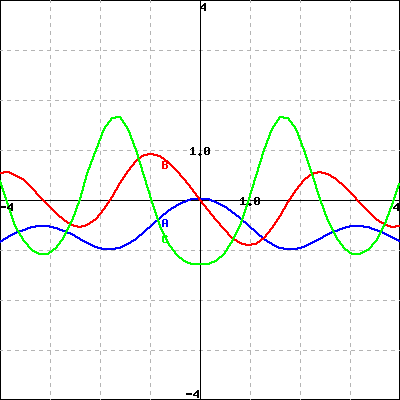
\includegraphics[width=0.8\linewidth]{/Volumes/WW_test/opt/webwork/courses/gage_demo/html/tmp/gif/gage-3105-setMAAtutorialprob8image1-.png}
 \par 
Identify the graphs A (blue), B( red) and C (green) as the graphs 
of a function and its
derivatives (click on the graph to see an enlarged image):\par 
\mbox{\parbox[t]{3ex}{\hrulefill}} is the graph of the function \par 
\mbox{\parbox[t]{3ex}{\hrulefill}} is the graph of the function's first derivative \par 
\mbox{\parbox[t]{3ex}{\hrulefill}} is the graph of the function's second derivative \par 

\par{\small{\it Answer(s) submitted:}
\vspace{-\parskip}\begin{itemize}
\item\begin{verbatim}\end{verbatim}
\item\begin{verbatim}\end{verbatim}
\item\begin{verbatim}\end{verbatim}
\end{itemize}} (incorrect)\par
%%%%%%%%%%%%%%%%%%%%%%%%%%%%%%%%%%%%%%%%%%%%%%%%%%%%%%%%%%%%%%%%%%%%%%%%%%%%%%%%
% WeBWorK Online Homework Delivery System
% Copyright � 2000-2007 The WeBWorK Project, http://openwebwork.sf.net/
% $CVSHeader: webwork2/conf/snippets/hardcopyProblemDivider.tex,v 1.3 2004/06/24 21:10:50 dpvc Exp $
% 
% This program is free software; you can redistribute it and/or modify it under
% the terms of either: (a) the GNU General Public License as published by the
% Free Software Foundation; either version 2, or (at your option) any later
% version, or (b) the "Artistic License" which comes with this package.
% 
% This program is distributed in the hope that it will be useful, but WITHOUT
% ANY WARRANTY; without even the implied warranty of MERCHANTABILITY or FITNESS
% FOR A PARTICULAR PURPOSE.  See either the GNU General Public License or the
% Artistic License for more details.
%%%%%%%%%%%%%%%%%%%%%%%%%%%%%%%%%%%%%%%%%%%%%%%%%%%%%%%%%%%%%%%%%%%%%%%%%%%%%%%%

\medskip
\goodbreak
\hrule
\nobreak
\smallskip
%% decoded old answers, saved. (keys = 
{\bf 9. {\footnotesize (1 pt) setMAAtutorial\-/ontheflygraphicsexample2.pg}}\newline \leavevmode\\\relax {\bf On-the-fly Graphics Example2}\leavevmode\\\relax \leavevmode\\\relax 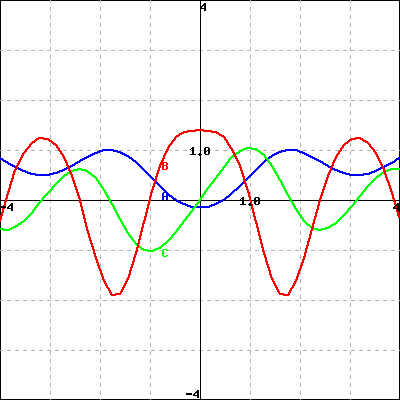
\includegraphics[width=0.8\linewidth]{/Volumes/WW_test/opt/webwork/courses/gage_demo/html/tmp/gif/gage-761-setMAAtutorialprob9image1-.png}
 \par 
Identify the graphs A (blue), B( red) and C (green) as the graphs of a function and its
derivatives (click on the graph to see an enlarged image):\par 
\mbox{\parbox[t]{3ex}{\hrulefill}} is the graph of the function \par 
\mbox{\parbox[t]{3ex}{\hrulefill}} is the graph of the function's first derivative \par 
\mbox{\parbox[t]{3ex}{\hrulefill}} is the graph of the function's second derivative \par 

\par{\small{\it Answer(s) submitted:}
\vspace{-\parskip}\begin{itemize}
\item\begin{verbatim}\end{verbatim}
\item\begin{verbatim}\end{verbatim}
\item\begin{verbatim}\end{verbatim}
\end{itemize}} (incorrect)\par
%%%%%%%%%%%%%%%%%%%%%%%%%%%%%%%%%%%%%%%%%%%%%%%%%%%%%%%%%%%%%%%%%%%%%%%%%%%%%%%%
% WeBWorK Online Homework Delivery System
% Copyright � 2000-2007 The WeBWorK Project, http://openwebwork.sf.net/
% $CVSHeader: webwork2/conf/snippets/hardcopyProblemDivider.tex,v 1.3 2004/06/24 21:10:50 dpvc Exp $
% 
% This program is free software; you can redistribute it and/or modify it under
% the terms of either: (a) the GNU General Public License as published by the
% Free Software Foundation; either version 2, or (at your option) any later
% version, or (b) the "Artistic License" which comes with this package.
% 
% This program is distributed in the hope that it will be useful, but WITHOUT
% ANY WARRANTY; without even the implied warranty of MERCHANTABILITY or FITNESS
% FOR A PARTICULAR PURPOSE.  See either the GNU General Public License or the
% Artistic License for more details.
%%%%%%%%%%%%%%%%%%%%%%%%%%%%%%%%%%%%%%%%%%%%%%%%%%%%%%%%%%%%%%%%%%%%%%%%%%%%%%%%

\medskip
\goodbreak
\hrule
\nobreak
\smallskip
%% decoded old answers, saved. (keys = 
 \end{multicols}
{\bf 10. {\footnotesize (1 pt) setMAAtutorial\-/staticgraphicsexample\-/staticgraphicsexample.pg}}\newline \leavevmode\\\relax {\bf Static graphics Example}\leavevmode\\\relax \leavevmode\\\relax This is a graph of the function \(F(x)\):
({\bf  Click on image for a larger view })
\par 
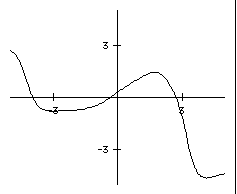
\includegraphics[width=0.2\linewidth]{/Volumes/WW_test/opt/webwork/courses/gage_demo/templates/setMAAtutorial/staticgraphicsexample/1.png}

\par 
Enter the letter of the graph below which corresponds to the transformation
of the function.

\par\begin{enumerate}
\item[\mbox{\parbox[t]{3ex}{\hrulefill}}1.] \(F(x/3)\)
\item[\mbox{\parbox[t]{3ex}{\hrulefill}}2.] \(-F(-x)\) 
\item[\mbox{\parbox[t]{3ex}{\hrulefill}}3.] \(F(3x)\)
\item[\mbox{\parbox[t]{3ex}{\hrulefill}}4.] \(5F(x)\)
\end{enumerate}



\par\smallskip\begin{center}\begin{tabular}{|c|c|c|c|} \hline
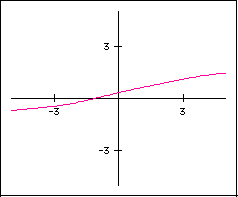
\includegraphics[width=0.2\linewidth]{/Volumes/WW_test/opt/webwork/courses/gage_demo/templates/setMAAtutorial/staticgraphicsexample/1-91734.png}
 &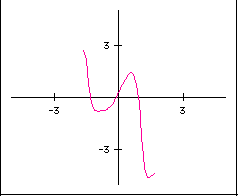
\includegraphics[width=0.2\linewidth]{/Volumes/WW_test/opt/webwork/courses/gage_demo/templates/setMAAtutorial/staticgraphicsexample/1-42639.png}
 &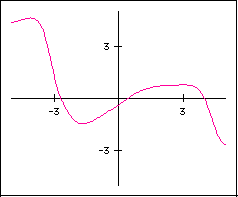
\includegraphics[width=0.2\linewidth]{/Volumes/WW_test/opt/webwork/courses/gage_demo/templates/setMAAtutorial/staticgraphicsexample/1-96355.png}
 &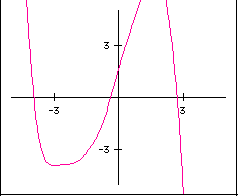
\includegraphics[width=0.2\linewidth]{/Volumes/WW_test/opt/webwork/courses/gage_demo/templates/setMAAtutorial/staticgraphicsexample/1-89540.png}
 \\ \hline 
A &B &C &D \\ \hline 

\end {tabular}\end{center}\par\smallskip
 \begin{multicols}{2}
\columnwidth=\linewidth
\par{\small{\it Answer(s) submitted:}
\vspace{-\parskip}\begin{itemize}
\item\begin{verbatim}\end{verbatim}
\item\begin{verbatim}\end{verbatim}
\item\begin{verbatim}\end{verbatim}
\item\begin{verbatim}\end{verbatim}
\end{itemize}} (incorrect)\par
%%%%%%%%%%%%%%%%%%%%%%%%%%%%%%%%%%%%%%%%%%%%%%%%%%%%%%%%%%%%%%%%%%%%%%%%%%%%%%%%
% WeBWorK Online Homework Delivery System
% Copyright � 2000-2007 The WeBWorK Project, http://openwebwork.sf.net/
% $CVSHeader: webwork2/conf/snippets/hardcopyProblemDivider.tex,v 1.3 2004/06/24 21:10:50 dpvc Exp $
% 
% This program is free software; you can redistribute it and/or modify it under
% the terms of either: (a) the GNU General Public License as published by the
% Free Software Foundation; either version 2, or (at your option) any later
% version, or (b) the "Artistic License" which comes with this package.
% 
% This program is distributed in the hope that it will be useful, but WITHOUT
% ANY WARRANTY; without even the implied warranty of MERCHANTABILITY or FITNESS
% FOR A PARTICULAR PURPOSE.  See either the GNU General Public License or the
% Artistic License for more details.
%%%%%%%%%%%%%%%%%%%%%%%%%%%%%%%%%%%%%%%%%%%%%%%%%%%%%%%%%%%%%%%%%%%%%%%%%%%%%%%%

\medskip
\goodbreak
\hrule
\nobreak
\smallskip
%% decoded old answers, saved. (keys = 
 \end{multicols}
{\bf 11. {\footnotesize (1 pt) setMAAtutorial\-/hermitegraphexample.pg}}\newline \leavevmode\\\relax {\bf Hermite polynomial graph example}\leavevmode\\\relax \leavevmode\\\relax \par 
We have developed other ways to specify graphs which are to be created 'on the fly'. 
All of these new methods consist of adding macro packages to WeBWorK.  Since they
do not require the core of WeBWorK to be changed, these enhancements can be added by
anyone using WeBWorK. 
\par 
 These two piecewise linear graphs were created by specifying the points at the nodes.
 \leavevmode\\\relax  Click on the graph to view a larger image.
\par 
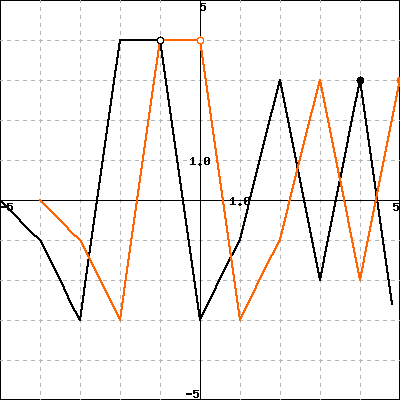
\includegraphics[width=0.3\linewidth]{/Volumes/WW_test/opt/webwork/courses/gage_demo/html/tmp/gif/gage-2913-setMAAtutorialprob11image1.png}

\par\hrulefill\par 
If the black function is written as \(f(x)\), then the orange function 
would be written as \(f(\) \mbox{\parbox[t]{10ex}{\hrulefill}} \()\).


\par\hrulefill\par 
This graph was created using a hermite spline by specifying points at


\par\smallskip\begin{center}\begin{tabular}{|c|c|c|c|c|c|c|c|c|c|} \hline

x &-4 &-3 &-2 &-1 &0 &1 &2 &3 &4 \\ \hline 

y &0 &1 &2 &0 &-1.5 &0.5 &-2 &1 &2 \\ \hline 

yp &0.1 &1 &0 &-2 &0 &1 &2 &-3 &1 \\ \hline 


\end {tabular}\end{center}\par\smallskip


\par 

\par\smallskip\begin{center}\begin{tabular}{|c|c|} \hline

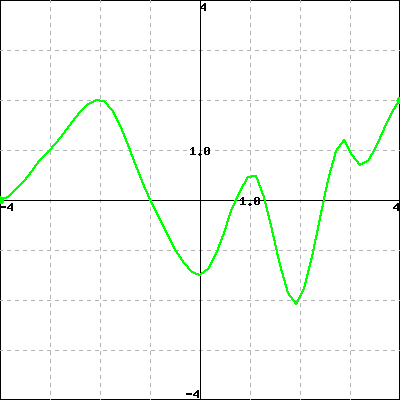
\includegraphics[width=0.3\linewidth]{/Volumes/WW_test/opt/webwork/courses/gage_demo/html/tmp/gif/gage-2913-setMAAtutorialprob11image2.png}
 &List the internal local minimum points \leavevmode\\\relax  in increasing order: \leavevmode\\\relax   \mbox{\parbox[t]{5ex}{\hrulefill}}  \mbox{\parbox[t]{5ex}{\hrulefill}}  \mbox{\parbox[t]{5ex}{\hrulefill}}  \\ \hline 


\end {tabular}\end{center}\par\smallskip


\par 

 \begin{multicols}{2}
\columnwidth=\linewidth
\par{\small{\it Answer(s) submitted:}
\vspace{-\parskip}\begin{itemize}
\item\begin{verbatim}\end{verbatim}
\item\begin{verbatim}\end{verbatim}
\item\begin{verbatim}\end{verbatim}
\item\begin{verbatim}\end{verbatim}
\end{itemize}} (incorrect)\par
%%%%%%%%%%%%%%%%%%%%%%%%%%%%%%%%%%%%%%%%%%%%%%%%%%%%%%%%%%%%%%%%%%%%%%%%%%%%%%%%
% WeBWorK Online Homework Delivery System
% Copyright � 2000-2007 The WeBWorK Project, http://openwebwork.sf.net/
% $CVSHeader: webwork2/conf/snippets/hardcopyProblemDivider.tex,v 1.3 2004/06/24 21:10:50 dpvc Exp $
% 
% This program is free software; you can redistribute it and/or modify it under
% the terms of either: (a) the GNU General Public License as published by the
% Free Software Foundation; either version 2, or (at your option) any later
% version, or (b) the "Artistic License" which comes with this package.
% 
% This program is distributed in the hope that it will be useful, but WITHOUT
% ANY WARRANTY; without even the implied warranty of MERCHANTABILITY or FITNESS
% FOR A PARTICULAR PURPOSE.  See either the GNU General Public License or the
% Artistic License for more details.
%%%%%%%%%%%%%%%%%%%%%%%%%%%%%%%%%%%%%%%%%%%%%%%%%%%%%%%%%%%%%%%%%%%%%%%%%%%%%%%%

\medskip
\goodbreak
\hrule
\nobreak
\smallskip
%% decoded old answers, saved. (keys = 
{\bf 12. {\footnotesize (1 pt) setMAAtutorial\-/htmllinksexample\-/htmllinksexample.pg}}\newline \leavevmode\\\relax {\bf HTML links example}\leavevmode\\\relax \leavevmode\\\relax This example shows how to link to resources outside the problem itself.
\par 
Linking to other web pages over the internet is easy. For example,
you can get more information about the buffon needle problem and how it is used by ants to find new nest sites  by linking to
 {\bf \underline{Ivars Peterson's column on the MAA site}}.
\par 

All of the files in the html directory of your WeBWorK course site can be read
by anyone with a web browser and the URL (the  address of the file). This is a good
place to put files that are referenced by more than one problem in your WeBWorK course.
\par 
Here is the link to 
the 
{\bf \underline{to the calculator page}} 
stored in the top level of the 
html directory of the tutorialCourse. 
\par 

Finally there are files, such as picture files, which are 
stored with the problem itself in the same directory. 
 \leavevmode\\\relax  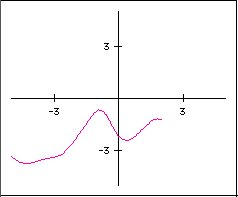
\includegraphics[width=0.8\linewidth]{/Volumes/WW_test/opt/webwork/courses/gage_demo/html/tmp/images/038962f0-1b3f-3fca-ac1f-64cd37a4f814___293a0dc9-0656-3fbd-9a21-ed6f6ef92bdc.png}
 

\par 
And the table below has three more graphs which are stored 
in the directory containing the current problem. \par 


\par\smallskip\begin{center}\begin{tabular}{|c|c|c|} \hline
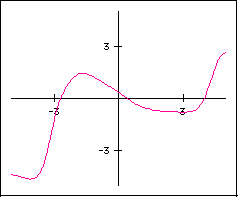
\includegraphics[width=0.2\linewidth]{/Volumes/WW_test/opt/webwork/courses/gage_demo/html/tmp/images/038962f0-1b3f-3fca-ac1f-64cd37a4f814___0eea18cb-31a0-37c0-9419-b1211999a78b.png}
 &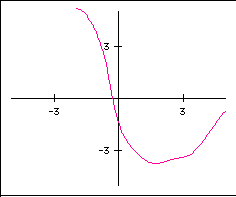
\includegraphics[width=0.2\linewidth]{/Volumes/WW_test/opt/webwork/courses/gage_demo/html/tmp/images/038962f0-1b3f-3fca-ac1f-64cd37a4f814___0d0696a5-99a2-32a8-8b41-e3c4e6168aa5.png}
 &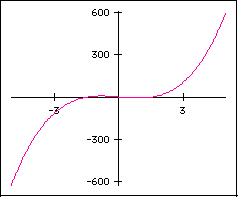
\includegraphics[width=0.2\linewidth]{/Volumes/WW_test/opt/webwork/courses/gage_demo/html/tmp/images/038962f0-1b3f-3fca-ac1f-64cd37a4f814___72b96c17-c4ed-35a2-aed9-168ecd7acf69.png}
 \\ \hline 

\end {tabular}\end{center}\par\smallskip
%%%%%%%%%%%%%%%%%%%%%%%%%%%%%%%%%%%%%%%%%%%%%%%%%%%%%%%%%%%%%%%%%%%%%%%%%%%%%%%%
% WeBWorK Online Homework Delivery System
% Copyright � 2000-2007 The WeBWorK Project, http://openwebwork.sf.net/
% $CVSHeader: webwork2/conf/snippets/hardcopyProblemDivider.tex,v 1.3 2004/06/24 21:10:50 dpvc Exp $
% 
% This program is free software; you can redistribute it and/or modify it under
% the terms of either: (a) the GNU General Public License as published by the
% Free Software Foundation; either version 2, or (at your option) any later
% version, or (b) the "Artistic License" which comes with this package.
% 
% This program is distributed in the hope that it will be useful, but WITHOUT
% ANY WARRANTY; without even the implied warranty of MERCHANTABILITY or FITNESS
% FOR A PARTICULAR PURPOSE.  See either the GNU General Public License or the
% Artistic License for more details.
%%%%%%%%%%%%%%%%%%%%%%%%%%%%%%%%%%%%%%%%%%%%%%%%%%%%%%%%%%%%%%%%%%%%%%%%%%%%%%%%

\medskip
\goodbreak
\hrule
\nobreak
\smallskip
%% decoded old answers, saved. (keys = 
{\bf 13. {\footnotesize (1 pt) setMAAtutorial\-/javascriptexample1.pg}}\newline \leavevmode\\\relax {\bf JavaScript Example 1}\leavevmode\\\relax \leavevmode\\\relax {\bf 13. {\footnotesize (1 pt) setMAAtutorial\-/javascriptexample1.pg}}\newline Find the derivative of the function f(x).  The windows below will tell
you the value of f for any input x. (I call this an "oracle function", since
if you ask, it will tell.)
\par 
\(f '( 0  )\) = \mbox{\parbox[t]{25ex}{\hrulefill}}
\par 
You may want to use a  
{\bf \underline{calculator}} 

to find the result.  
 You can also enter numerical expressions and have 
 WeBWorK do the calculations for you.

 \fbox{ The java Script calculator was displayed here
                    }\par{\small{\it Answer(s) submitted:}
\vspace{-\parskip}\begin{itemize}
\item\begin{verbatim}\end{verbatim}
\end{itemize}} (incorrect)\par
%%%%%%%%%%%%%%%%%%%%%%%%%%%%%%%%%%%%%%%%%%%%%%%%%%%%%%%%%%%%%%%%%%%%%%%%%%%%%%%%
% WeBWorK Online Homework Delivery System
% Copyright � 2000-2007 The WeBWorK Project, http://openwebwork.sf.net/
% $CVSHeader: webwork2/conf/snippets/hardcopyProblemDivider.tex,v 1.3 2004/06/24 21:10:50 dpvc Exp $
% 
% This program is free software; you can redistribute it and/or modify it under
% the terms of either: (a) the GNU General Public License as published by the
% Free Software Foundation; either version 2, or (at your option) any later
% version, or (b) the "Artistic License" which comes with this package.
% 
% This program is distributed in the hope that it will be useful, but WITHOUT
% ANY WARRANTY; without even the implied warranty of MERCHANTABILITY or FITNESS
% FOR A PARTICULAR PURPOSE.  See either the GNU General Public License or the
% Artistic License for more details.
%%%%%%%%%%%%%%%%%%%%%%%%%%%%%%%%%%%%%%%%%%%%%%%%%%%%%%%%%%%%%%%%%%%%%%%%%%%%%%%%

\medskip
\goodbreak
\hrule
\nobreak
\smallskip
%% decoded old answers, saved. (keys = 
{\bf 14. {\footnotesize (1 pt) setMAAtutorial\-/javascriptexample2.pg}}\newline \leavevmode\\\relax {\bf JavaScript Example 2}\leavevmode\\\relax \leavevmode\\\relax {\bf 14. {\footnotesize (1 pt) setMAAtutorial\-/javascriptexample2.pg}}\newline Find the derivative of the function f(x).  The windows below will tell
you the value of f for any input x. (I call this an "oracle function", since
if you ask, it will tell.)
\par 
\(f'( 1  )\) = \mbox{\parbox[t]{25ex}{\hrulefill}}
\par 
You may want to use a  
{\bf \underline{calculator}} 

to find the result.  You can also enter numerical expressions and 
have WeBWorK do the calculations for you.

 \fbox{ The java Script calculator was displayed here
                    }\par{\small{\it Answer(s) submitted:}
\vspace{-\parskip}\begin{itemize}
\item\begin{verbatim}\end{verbatim}
\end{itemize}} (incorrect)\par
%%%%%%%%%%%%%%%%%%%%%%%%%%%%%%%%%%%%%%%%%%%%%%%%%%%%%%%%%%%%%%%%%%%%%%%%%%%%%%%%
% WeBWorK Online Homework Delivery System
% Copyright � 2000-2007 The WeBWorK Project, http://openwebwork.sf.net/
% $CVSHeader: webwork2/conf/snippets/hardcopyProblemDivider.tex,v 1.3 2004/06/24 21:10:50 dpvc Exp $
% 
% This program is free software; you can redistribute it and/or modify it under
% the terms of either: (a) the GNU General Public License as published by the
% Free Software Foundation; either version 2, or (at your option) any later
% version, or (b) the "Artistic License" which comes with this package.
% 
% This program is distributed in the hope that it will be useful, but WITHOUT
% ANY WARRANTY; without even the implied warranty of MERCHANTABILITY or FITNESS
% FOR A PARTICULAR PURPOSE.  See either the GNU General Public License or the
% Artistic License for more details.
%%%%%%%%%%%%%%%%%%%%%%%%%%%%%%%%%%%%%%%%%%%%%%%%%%%%%%%%%%%%%%%%%%%%%%%%%%%%%%%%

\medskip
\goodbreak
\hrule
\nobreak
\smallskip
%% decoded old answers, saved. (keys = 
{\bf 15. {\footnotesize (1 pt) setMAAtutorial\-/vectorfieldexample.pg}}\newline  \end{multicols}


Match the following equations with their direction field. 
Clicking on each picture will give you an
enlarged view.  While you can probably solve this problem by guessing,
it is useful to try to predict characteristics of the direction field
and then match them to the picture.
\par 
Here are some handy characteristics to start with --
you will develop more as you practice.
\par 

\begin{enumerate}
\item[A.] Set y equal to zero and look at how the derivative behaves along the x axis.
\item[B.] Do the same for the y axis by setting x equal to 0
\item[C.] Consider the curve in the plane defined by setting y'=0
   -- this should correspond to the points in the picture where the
   slope is zero.
\item[D.] Setting y' equal to a constant other than zero gives the curve of points
   where the slope is that
   constant.  These are called isoclines, and can be used to construct the
   direction field picture by hand.
\end{enumerate}

        

        
\par\begin{enumerate}
\item[\mbox{\parbox[t]{3ex}{\hrulefill}}1.] \(y'= 2y + x^2e^{2x}\)
\item[\mbox{\parbox[t]{3ex}{\hrulefill}}2.] \(y'= e^{-x} + 2y\)
\item[\mbox{\parbox[t]{3ex}{\hrulefill}}3.] \(y'= 2\sin(x) + 1 + y\)
\item[\mbox{\parbox[t]{3ex}{\hrulefill}}4.] \(y'= -2 + x - y\)
\end{enumerate}


\par 
        
\par\smallskip\begin{center}\begin{tabular}{|c|c|} \hline
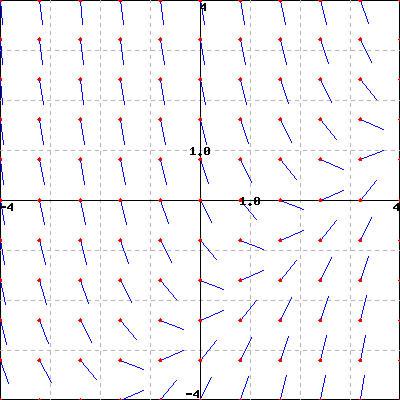
\includegraphics[width=0.3\linewidth]{/Volumes/WW_test/opt/webwork/courses/gage_demo/html/tmp/gif/gage-4604-setMAAtutorialprob15image1.png}
&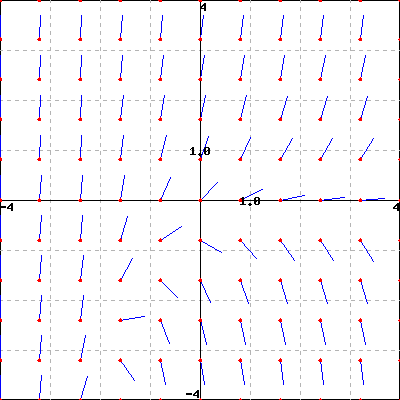
\includegraphics[width=0.3\linewidth]{/Volumes/WW_test/opt/webwork/courses/gage_demo/html/tmp/gif/gage-4604-setMAAtutorialprob15image2.png}
\\ \hline 
 A 
& B 
\\ \hline 
\end {tabular}\end{center}\par\smallskip

       
\par\smallskip\begin{center}\begin{tabular}{|c|c|} \hline
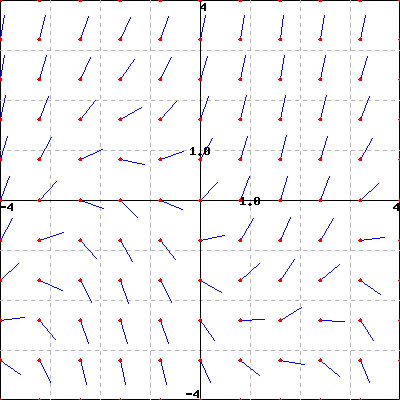
\includegraphics[width=0.3\linewidth]{/Volumes/WW_test/opt/webwork/courses/gage_demo/html/tmp/gif/gage-4604-setMAAtutorialprob15image3.png}
&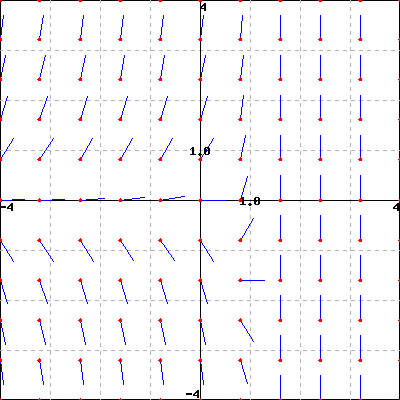
\includegraphics[width=0.3\linewidth]{/Volumes/WW_test/opt/webwork/courses/gage_demo/html/tmp/gif/gage-4604-setMAAtutorialprob15image4.png}
\\ \hline 
 C 
& D 
\\ \hline 
\end {tabular}\end{center}\par\smallskip

       
 \begin{multicols}{2}
\columnwidth=\linewidth


\par{\small{\it Answer(s) submitted:}
\vspace{-\parskip}\begin{itemize}
\item\begin{verbatim}\end{verbatim}
\item\begin{verbatim}\end{verbatim}
\item\begin{verbatim}\end{verbatim}
\item\begin{verbatim}\end{verbatim}
\end{itemize}} (incorrect)\par
%%%%%%%%%%%%%%%%%%%%%%%%%%%%%%%%%%%%%%%%%%%%%%%%%%%%%%%%%%%%%%%%%%%%%%%%%%%%%%%%
% WeBWorK Online Homework Delivery System
% Copyright � 2000-2007 The WeBWorK Project, http://openwebwork.sf.net/
% $CVSHeader: webwork2/conf/snippets/hardcopyProblemDivider.tex,v 1.3 2004/06/24 21:10:50 dpvc Exp $
% 
% This program is free software; you can redistribute it and/or modify it under
% the terms of either: (a) the GNU General Public License as published by the
% Free Software Foundation; either version 2, or (at your option) any later
% version, or (b) the "Artistic License" which comes with this package.
% 
% This program is distributed in the hope that it will be useful, but WITHOUT
% ANY WARRANTY; without even the implied warranty of MERCHANTABILITY or FITNESS
% FOR A PARTICULAR PURPOSE.  See either the GNU General Public License or the
% Artistic License for more details.
%%%%%%%%%%%%%%%%%%%%%%%%%%%%%%%%%%%%%%%%%%%%%%%%%%%%%%%%%%%%%%%%%%%%%%%%%%%%%%%%

\medskip
\goodbreak
\hrule
\nobreak
\smallskip
%% decoded old answers, saved. (keys = 
{\bf 16. {\footnotesize (1 pt) setMAAtutorial\-/conditionalquestionexample.pg}}\newline \leavevmode\\\relax {\bf Conditional questions example}\leavevmode\\\relax \leavevmode\\\relax If \(f(x) = 8 x + 14\), find \(f'( 6 )\).
\leavevmode\\\relax  \leavevmode\\\relax  \mbox{\parbox[t]{5ex}{\hrulefill}}
\leavevmode\\\relax 

\par{\small{\it Answer(s) submitted:}
\vspace{-\parskip}\begin{itemize}
\item\begin{verbatim}\end{verbatim}
\end{itemize}} (incorrect)\par
%%%%%%%%%%%%%%%%%%%%%%%%%%%%%%%%%%%%%%%%%%%%%%%%%%%%%%%%%%%%%%%%%%%%%%%%%%%%%%%%
% WeBWorK Online Homework Delivery System
% Copyright � 2000-2007 The WeBWorK Project, http://openwebwork.sf.net/
% $CVSHeader: webwork2/conf/snippets/hardcopyProblemDivider.tex,v 1.3 2004/06/24 21:10:50 dpvc Exp $
% 
% This program is free software; you can redistribute it and/or modify it under
% the terms of either: (a) the GNU General Public License as published by the
% Free Software Foundation; either version 2, or (at your option) any later
% version, or (b) the "Artistic License" which comes with this package.
% 
% This program is distributed in the hope that it will be useful, but WITHOUT
% ANY WARRANTY; without even the implied warranty of MERCHANTABILITY or FITNESS
% FOR A PARTICULAR PURPOSE.  See either the GNU General Public License or the
% Artistic License for more details.
%%%%%%%%%%%%%%%%%%%%%%%%%%%%%%%%%%%%%%%%%%%%%%%%%%%%%%%%%%%%%%%%%%%%%%%%%%%%%%%%

\medskip
\goodbreak
\hrule
\nobreak
\smallskip
%% decoded old answers, saved. (keys = 
{\bf 17. {\footnotesize (1 pt) setMAAtutorial\-/javaappletexample.pg}}\newline \leavevmode\\\relax {\bf Java applet example}\leavevmode\\\relax \leavevmode\\\relax \par 
This problem illustrates how you can embed Java applet code in a WeBWorK example
to create an interactive homework problem that could never be provided by a text book.
\par 
WeBWorK can use existing {\bf  javaScript}  and {\bf  Java } 
code to augment its capabilities.
\par\hrulefill\par 

 \fbox{ The java applet was displayed here
                    }\par 
The graph above represents the function
\[f(x) = x^2 + a x +b\]
where \(a\) and \(b\) are parameters. \par 

For each value of \(a\) find the value of \(b\) which 
makes the graph just touch the x-axis.  
\leavevmode\\\relax 
if a= 1 then \mbox{\parbox[t]{5ex}{\hrulefill}}\leavevmode\\\relax 
if a= 1.5 then \mbox{\parbox[t]{5ex}{\hrulefill}}\leavevmode\\\relax 
if a= -1.5 then \mbox{\parbox[t]{5ex}{\hrulefill}} \par 

Does this relationship between a and b specify b as a function of a?
 \mbox{\parbox[t]{3ex}{\hrulefill}} (Yes or No)\leavevmode\\\relax 

Does this relationship between a and b specify a as a function of b?
 \mbox{\parbox[t]{3ex}{\hrulefill}} (Yes or No)\leavevmode\\\relax 

Write a formula for calculating this value of \(b\) from \(a\).\leavevmode\\\relax 
b = \mbox{\parbox[t]{20ex}{\hrulefill}}

\par{\small{\it Answer(s) submitted:}
\vspace{-\parskip}\begin{itemize}
\item\begin{verbatim}\end{verbatim}
\item\begin{verbatim}\end{verbatim}
\item\begin{verbatim}\end{verbatim}
\item\begin{verbatim}\end{verbatim}
\item\begin{verbatim}\end{verbatim}
\item\begin{verbatim}\end{verbatim}
\end{itemize}} (incorrect)\par
%% decoded old answers, saved. (keys = 
 \end{multicols}


\noindent {\tiny Generated by \copyright WeBWorK, http://webwork.maa.org, Mathematical Association of America}

 \begin{multicols}{2}
\columnwidth=\linewidth


%%%%%%%%%%%%%%%%%%%%%%%%%%%%%%%%%%%%%%%%%%%%%%%%%%%%%%%%%%%%%%%%%%%%%%%%%%%%%%%%
% WeBWorK Online Homework Delivery System
% Copyright � 2000-2007 The WeBWorK Project, http://openwebwork.sf.net/
% $CVSHeader: webwork2/conf/snippets/hardcopyPostamble.tex,v 1.2 2003/12/09 01:12:29 sh002i Exp $
% 
% This program is free software; you can redistribute it and/or modify it under
% the terms of either: (a) the GNU General Public License as published by the
% Free Software Foundation; either version 2, or (at your option) any later
% version, or (b) the "Artistic License" which comes with this package.
% 
% This program is distributed in the hope that it will be useful, but WITHOUT
% ANY WARRANTY; without even the implied warranty of MERCHANTABILITY or FITNESS
% FOR A PARTICULAR PURPOSE.  See either the GNU General Public License or the
% Artistic License for more details.
%%%%%%%%%%%%%%%%%%%%%%%%%%%%%%%%%%%%%%%%%%%%%%%%%%%%%%%%%%%%%%%%%%%%%%%%%%%%%%%%

\end{multicols}
\vfill
\end{document}
